%%%%%%%%%%%%%%%%%%%%%%%%%%%%%%%%%%%%%%%%%
% Developer CV
% LaTeX Template
% Version 1.0 (28/1/19)
%
% This template originates from:
% http://www.LaTeXTemplates.com
%
% Authors:
% Jan Vorisek (jan@vorisek.me)
% Based on a template by Jan Küster (info@jankuester.com)
% Modified for LaTeX Templates by Vel (vel@LaTeXTemplates.com)
%
% License:
% The MIT License (see included LICENSE file)
%
%%%%%%%%%%%%%%%%%%%%%%%%%%%%%%%%%%%%%%%%%

%----------------------------------------------------------------------------------------
%	PACKAGES AND OTHER DOCUMENT CONFIGURATIONS
%----------------------------------------------------------------------------------------

\documentclass[9pt]{developercv} % Default font size, values from 8-12pt are recommended
\usepackage{graphicx, float}

%----------------------------------------------------------------------------------------

\begin{document}

%----------------------------------------------------------------------------------------
%	TITLE AND CONTACT INFORMATION
%-------------------------------------------------------------------------------------
\begin{minipage}[t]{0.25\textwidth} % 27.5% of the page width for the second row of icons
	\vspace{-\baselineskip} % Required for vertically aligning minipages
   %	\begin{figure}[h]
      \centering
       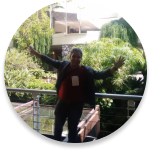
\includegraphics[width=0.8\linewidth]{FOTAJB.png}
    %\end{figure}
	
\end{minipage}\hfill
\begin{minipage}[t]{0.45\textwidth} % 45% of the page width for name
	\vspace{-\baselineskip} % Required for vertically aligning minipages
	
	% If your name is very short, use just one of the lines below
	% If your name is very long, reduce the font size or make the minipage wider and reduce the others proportionately
	\colorbox{black}{{\HUGE\textcolor{white}{\textbf{\MakeUppercase{Jonathan}}}}} % First name
	
	\colorbox{black}{{\HUGE\textcolor{white}{\textbf{\MakeUppercase{Batista}}}}} % Last name
	
	\vspace{6pt}
	
	{\huge Undergraduate Student (USP)} % Career or current job title
\end{minipage}
\begin{minipage}[t]{0.275\textwidth} % 27.5% of the page width for the first row of icons
	\vspace{-\baselineskip} % Required for vertically aligning minipages
	
	% The first parameter is the FontAwesome icon name, the second is the box size and the third is the text
	% Other icons can be found by referring to fontawesome.pdf (supplied with the template) and using the word after \fa in the command for the icon you want
	\icon{MapMarker}{12}{\href{https://jonathanbff.github.io/}{Personal Website}}\\
	\icon{Phone}{12}{+55 16 991537025}\\
	\icon{At}{12}{\href{mailto:jonathanbf@usp.br}{jonathanbf@usp.br}}\\	
	\icon{Linkedin}{12}{\href{https://www.linkedin.com/in/jonathan-batista-ferreira-1b951b150/}{Jonathan Batista}}\\
	\icon{Github}{12}{\href{github.com/jonathanbff}{jonathanbff}}
\end{minipage}


\vspace{0.5cm}

%----------------------------------------------------------------------------------------
%	INTRODUCTION, SKILLS AND TECHNOLOGIES
%----------------------------------------------------------------------------------------

\cvsect{Intro}

\begin{minipage}[t]{0.4\textwidth} % 40% of the page width for the introduction text
	\vspace{-\baselineskip} % Required for vertically aligning minipages
	
	{ Hello World, my name is Jonathan Batista I'm a Undergraduate Student from University of São Paulo (USP), 19 years old and actually i'm being former director of the group Neuron Data Science and Artificial Intelligence, that does works with Workshops, Speeches and Events in Data Science and programming }\\ % Dummy text
\end{minipage}
\hfill % Whitespace between
\begin{minipage}[t]{0.5\textwidth} % 50% of the page for the skills bar chart
	\vspace{-\baselineskip} % Required for vertically aligning minipages
	\begin{barchart}{5.5}
		\baritem{Python}{100}
		\baritem{Data Analysis}{90}
		\baritem{Machine Learning Models }{60}
		\baritem{Java and C}{40}
		\baritem{R}{30}
		\baritem{Office }{100}
	\end{barchart}
\end{minipage}

\begin{center}
	\bubbles{5/sklearn, 6/Pandas, 4/Numpy, 2/TsFlow, 4/Seaborn}
\end{center}

%----------------------------------------------------------------------------------------
%	EXPERIENCE
%----------------------------------------------------------------------------------------

\cvsect{Experience}

\begin{entrylist}
	\entry
		{2014 -- 2018\\\footnotesize{part time}}
		{OBMEP - Math Scientific Initiation (Jr.)}
		{OBMEP - Math Faculty (USP)}
		{Math Scientific Initiation, for Awarded students of the National Math Olympics\\ \texttt{Math}\slashsep\texttt{Programming}\slashsep\texttt{\LaTeX}}
	\entry
		{2017 -- 2019\\\footnotesize{part time}}
		{Neuroscience Scientific Initiation (Jr.)}
		{Ribeirão Preto Medical School - USP}
		{Neuroscience Scientific Initiation that has promoted scientific diffusion and Lab essays \\ \texttt{Scientific Methodology}\slashsep\texttt{Communication}}
	\entry
		{2019 - 2020\\\footnotesize{part time}}
		{Co-founder and General Director}
		{Neuron Data Science and Artificial Intelligence }
		{Co-founder and Actually General Director of the group Neuron Data Science and Artificial Intelligence doing Data Science Projects and material to diffuse Data Science and Machine Learning \\ \texttt{Data Science}\slashsep\texttt{Machine Learning}\slashsep\texttt{Python}}
\end{entrylist}

%----------------------------------------------------------------------------------------
%	EDUCATION
%----------------------------------------------------------------------------------------

\cvsect{Education}

\begin{entrylist}
	\entry
		{2020}
		{Machine Learning Scientific Initiation}
		{IME -Univeristy of São Paulo (USP)}
		{The Machine Learning Scientific Initiation, is a student group in Machine Learning, where ungrad students learn statics and programming skills of Machine Learning every week from post-degree students, papers/books and teacher orientation }
	\entry
		{2020 -- 2024}
		{Bachelor's Degree}
		{Univeristy of São Paulo (USP)}
		{The Molecular Sciences Course (CCM) aims to train researchers with a multidisciplinary view in scientific and applied areas. In the first semesters, the student has a broad view of several scientific areas (Biology, Chemistry, Physics, Mathematics and Computation). In the rest of the course, the student develops a project in his area of interest, with the help of an advisor. At this stage, the student has complete freedom as to the choice of his curriculum, by creating an innovative project in science and technology, which includes academic research or Business Project.}
\end{entrylist}

%----------------------------------------------------------------------------------------
%	ADDITIONAL INFORMATION
%----------------------------------------------------------------------------------------

\begin{minipage}[t]{0.3\textwidth}
	\vspace{-\baselineskip} % Required for vertically aligning minipages

	\cvsect{Languages}
	
	\textbf{English} - proficient\\
	\textbf{Portuguese} - native\\
	\textbf{Spanish} - proficient 
\end{minipage}
\hfill
\begin{minipage}[t]{0.3\textwidth}
	\vspace{-\baselineskip} % Required for vertically aligning minipages
	
	\cvsect{Hobbies}
	
	I like to play RPG like D$\&$D, Sci-fi Books, video games, listening to podcasts and being part of Hackathons
\end{minipage}
\hfill
\begin{minipage}[t]{0.3\textwidth}
	\vspace{-\baselineskip} % Required for vertically aligning minipages
	
	\cvsect{Non profit}
	
	Blood Donor, Voluntary Math Teacher at a college prep course
\end{minipage}


%----------------------------------------------------------------------------------------

\end{document}
